\documentclass[12pt]{article}

\usepackage[margin=1in]{geometry}
\usepackage[T1]{fontenc}
\usepackage{amsmath,amssymb,mathtools}
\usepackage{newtxtext,newtxmath}
\usepackage{microtype}
\usepackage{xcolor}
\usepackage{tikz}
\usepackage{lineno}
\usepackage{setspace}
\usepackage[hidelinks]{hyperref}

\usetikzlibrary{arrows.meta,positioning}
\setstretch{1.48}
\linenumbers
\setlength{\parindent}{1.2em}
\setlength{\parskip}{0pt}
\setlength{\emergencystretch}{2em}

\newcommand{\C}{\mathbb C}
\newcommand{\R}{\mathbb R}
\newcommand{\ee}{\mathrm e}
\newcommand{\ii}{\mathrm i}

\title{\bfseries One quantum return record permits every future return probability}
\author{Michael Haufschild\\[2pt]\small Independent researcher\\
\small \texttt{haufschildmichael@gmail.com}}
\date{28 July 2026}

\begin{document}
\maketitle

\noindent\textbf{Long-time quantum behaviour is increasingly inferred from
shorter records. Here we determine a sharp limit for survival probability,
a direct diagnostic of recurrence and Loschmidt zeros. For every target
time \(T>0\), observation horizon \(0\leq H<T\), precision \(\delta>0\)
and finite moment order \(m\), we construct one fixed normalized state, one
fixed return projector and a continuum of finite nonnegative self-adjoint
Hamiltonians labelled by \(p\in[0,1]\). All Hamiltonians are unitarily
equivalent and therefore have exactly the same spectrum. Their
return-probability histories lie within \(\delta\) of one common record
throughout \([-H,H]\), and the fixed state has identical energy moments
through order \(m\). Nevertheless, at \(T\) its return probability under
the Hamiltonian labelled by \(p\) is exactly \(p\). Thus one protocol, one
spectrum and one record permit every possible return probability, including
perfect revival and exact orthogonality. An equivalent representation uses
one permutation-invariant uniform-field qubit Hamiltonian and different
symmetric pure preparations. For every \(p\in[0,1]\), the fixed-protocol
Hamiltonian can moreover be chosen tridiagonal: an exact nearest-neighbour
one-particle chain and the one-excitation block of a
particle-number-preserving spin chain. At perfect return the chain is a
Jacobi block plus an uncoupled diagonal spectator block, and a rigidity
theorem proves that every tridiagonal realization of this endpoint must
contain a zero path coupling; every less-than-perfect probability has a
connected representative. Its canonical lift to every fermion number
has a complete Slater eigenbasis; all members share
the same many-body subset-sum spectrum in every sector. The discrepancy is
exactly a sine power and decays exponentially on every strict pre-target
window. A Vandermonde converse proves minimum spectral support, and every
forecaster has worst-case terminal error at least one half.}

\section*{The recurrence question}

An isolated finite quantum system eventually revisits its initial
configuration. Recurrences have been observed in an isolated many-body gas
\cite{Rauer2018}; their times are the subject of new sharp bounds
\cite{KotowskiOszmaniec2026,GuptaShort2026} and proposed multiqubit tests
\cite{Karimi2026}. At the opposite extreme, a zero of the survival amplitude
means that the evolved state is exactly orthogonal to its initial state.
Real-time Loschmidt zeros are also used as finite-size indicators of
dynamical quantum phase transitions
\cite{Heyl2018,Zhou2021,Novotny2026}.

Experiments rarely reach the longest relevant times. Forecasting and
spectral-recovery methods therefore infer later observables from shorter
records \cite{Sornsaeng2024,Valls2026}. Their guarantees require structure,
such as sparse and separated Bohr frequencies. General quantum measurement
timelines can demand extreme precision for extrapolation and can display
``fog banks'' of complete future uncertainty \cite{Manos2026}. Hamiltonian
learning has complementary access-dependent lower bounds
\cite{ChenLi2026}. These results make a more restrictive recurrence question
natural: how much can one directly observed survival record leave
undetermined when every candidate is finite, pure, bounded below, and
evolves under one shared Hamiltonian?

For a normalized state \(\psi\) and self-adjoint Hamiltonian \(K\), define
\begin{equation}
 A(t)=\langle\psi,\ee^{\ii tK}\psi\rangle,\qquad
 P(t)=|A(t)|^2 .
\label{eq:survival}
\end{equation}
Here \(P(t)\) is the probability that a projection onto the initial state
succeeds at time \(t\). We ask what values \(P(T)\) remain compatible with a
finite-precision record of \(P(t)\) on the complete interval
\([-H,H]\).

\section*{A continuum of clocks on one Hamiltonian}

Fix \(n\geq1\) and first take \(T=1\). Use the \(n+1\) distinct
nonnegative energies
\begin{equation}
 E_j=\pi j,\qquad 0\leq j\leq n,
\label{eq:energies}
\end{equation}
and the fair-binomial weights
\begin{equation}
 q_j=2^{-n}{n\choose j}.
\label{eq:fullweight}
\end{equation}
Their survival amplitude is
\begin{equation}
 A_0(t)=\sum_{j=0}^{n}q_j\ee^{\ii\pi jt}
 =\left(\frac{1+\ee^{\ii\pi t}}2\right)^n .
\label{eq:A0}
\end{equation}

Now condition the same distribution on the parity class of \(n\):
\begin{equation}
 r_j=q_j\bigl[1+(-1)^{n-j}\bigr].
\label{eq:parityweight}
\end{equation}
The weights are twice \(q_j\) when \(j\equiv n\pmod2\) and zero otherwise;
they are nonnegative and sum to one. Their amplitude is
\begin{equation}
 A_1(t)=A_0(t)+
 \left(\frac{\ee^{\ii\pi t}-1}{2}\right)^n .
\label{eq:A1}
\end{equation}
Binomial states and their even--odd projections are established quantum
optical states \cite{Stoler1985,Zhang2009}. The advance here is not their
definition, but the exact continuum, moment and optimality law that follows
from placing them in a common recurrence problem.

For every \(p\in[0,1]\), interpolate the spectral weights by
\begin{equation}
 w_{p,j}=(1-\sqrt p)\,q_j+\sqrt p\,r_j.
\label{eq:interpolation}
\end{equation}
Every \(w_p\) is a probability distribution. On \(\C^{n+1}\), let \(K\) be
diagonal with entries \(E_j\), and let the \(p\)-clock be the pure state
\begin{equation}
 |\psi_p\rangle=\sum_{j=0}^{n}\sqrt{w_{p,j}}\,|j\rangle .
\label{eq:state}
\end{equation}
Thus all clocks are normalized, share one finite nonnegative self-adjoint
Hamiltonian, and differ only in preparation. Their amplitudes obey
\begin{equation}
 A_p(t)=A_0(t)+\sqrt p
 \left(\frac{\ee^{\ii\pi t}-1}{2}\right)^n .
\label{eq:Ap}
\end{equation}
At the target time,
\begin{equation}
 A_p(1)=\sqrt p\,(-1)^n,\qquad P_p(1)=p.
\label{eq:allfutures}
\end{equation}
One finite Hamiltonian therefore realizes the entire probability interval,
from \(P_0(1)=0\) to \(P_1(1)=1\).

\section*{One homogeneous qubit Hamiltonian}

The shared Hamiltonian has a direct many-qubit realization with no
engineered couplings. On \(n\) qubits define the uniform onsite field
\begin{equation}
 H_{\rm u}=\frac{\pi}{T}\sum_{a=1}^{n}
 |1\rangle\langle1|_a .
\label{eq:uniformfield}
\end{equation}
It is invariant under every permutation of the qubits, hence in particular
under lattice translations for any chosen periodic ordering. Let
\[
 |D_j^{(n)}\rangle={n\choose j}^{-1/2}
 \sum_{\substack{S\subseteq\{1,\ldots,n\}\\|S|=j}}|S\rangle
\]
be the normalized symmetric Dicke state with \(j\) excitations, and set
\begin{equation}
 |\Psi_p\rangle=\sum_{j=0}^{n}\sqrt{w_{p,j}}\,
 |D_j^{(n)}\rangle .
\label{eq:symmetricqubitstate}
\end{equation}
The Dicke states are orthonormal eigenvectors of \(H_{\rm u}\) with
energies \(\pi j/T\). Therefore \(|\Psi_p\rangle\) is normalized and
\[
 \langle\Psi_p|\ee^{\ii tH_{\rm u}}|\Psi_p\rangle
 =\sum_{j=0}^{n}w_{p,j}\ee^{\ii\pi jt/T}=A_p(t).
\]
All moment, finite-window and terminal identities consequently hold in one
fixed permutation-invariant, noninteracting qubit Hamiltonian. This
realization varies the symmetric preparation with \(p\); the next section
instead fixes preparation and measurement while varying isospectral
Hamiltonian eigenvectors.

\section*{One fixed protocol and one fixed spectrum}

The preparation dependence can be removed exactly. Fix the normalized
reference basis state \(|\phi\rangle=|0\rangle\in\C^{n+1}\). For every \(p\), choose a
unitary \(U_p\) satisfying
\[
 U_p|\phi\rangle=|\psi_p\rangle,
\]
and define
\begin{equation}
 \widetilde K_p=U_p^\dagger K U_p,\qquad
 |\phi_p(t)\rangle=U_p^\dagger|\psi_p(t)\rangle .
\label{eq:unitarytransport}
\end{equation}
Every \(\widetilde K_p\) is self-adjoint and nonnegative. They are all
unitarily equivalent to \(K\), so their spectra---including
multiplicities---are identical. The initial state and its return projector
\(|\phi\rangle\langle\phi|\) no longer depend on \(p\), while
\begin{equation}
 \langle\phi|\phi_p(t)\rangle
 =\langle\psi_p|\psi_p(t)\rangle=A_p(t).
\label{eq:fixedprotocol}
\end{equation}
Moreover,
\[
 \langle\phi|\widetilde K_p^{\,k}|\phi\rangle
 =\sum_{j=0}^{n}w_{p,j}E_j^k.
\]
Thus the moment identities, finite-window agreement and every terminal
probability survive with one fixed preparation, one fixed measurement and
one explicit common spectrum. Only the Hamiltonian eigenvectors vary.

\section*{Nearest-neighbour realization}

The isospectral ambiguity is not an artefact of dense matrices. For
\(0\leq p<1\), every weight \(w_{p,j}\) is strictly positive. Consider the
Krylov vectors
\[
 |\psi_p\rangle,\ K|\psi_p\rangle,\ldots,K^n|\psi_p\rangle.
\]
They are linearly independent: if
\(\sum_{k=0}^{n}c_kK^k|\psi_p\rangle=0\), its \(j\)th energy coordinate
gives
\[
 \sqrt{w_{p,j}}\sum_{k=0}^{n}c_kE_j^k=0.
\]
Strict positivity removes the square root, and the distinct \(E_j\) make
the remaining Vandermonde system invertible.

Apply Gram--Schmidt in this order, obtaining an orthonormal basis
\(\{|b_k^{(p)}\rangle\}_{k=0}^{n}\) with
\(|b_0^{(p)}\rangle=|\psi_p\rangle\). The nested Krylov spans satisfy
\[
 K\,\mathrm{span}\{b_0^{(p)},\ldots,b_j^{(p)}\}
 \subseteq
 \mathrm{span}\{b_0^{(p)},\ldots,b_{j+1}^{(p)}\}.
\]
Self-adjointness then gives
\begin{equation}
 \langle b_i^{(p)}|K|b_j^{(p)}\rangle=0
 \quad\text{whenever}\quad |i-j|>1.
\label{eq:tridiagonal}
\end{equation}
Choosing \(U_p|j\rangle=|b_j^{(p)}\rangle\) in
equation~\eqref{eq:unitarytransport} makes \(\widetilde K_p\)
tridiagonal in the fixed site basis, while retaining the fixed endpoint
state \(|0\rangle\), the full spectrum and the same return probability.
Thus every terminal probability below one occurs in an exact
nearest-neighbour one-particle chain.

The perfect-return endpoint has zero weights and therefore is not cyclic,
but locality does not fail. Choose \(n=2q+1\). The occupied odd-energy
levels and unoccupied even-energy levels each number \(q+1\). Apply the
same Krylov construction only to the positive odd-level weights. It gives
a \((q+1)\)-site Jacobi block whose first basis vector is
\(|\psi_1\rangle\). Place the unused even-energy eigenvectors in a diagonal
spectator block and order the active block before the spectator block:
\begin{equation}
 \widetilde K_1=
 \begin{pmatrix}
   J_{\rm odd}&0\\
   0&D_{\rm even}
 \end{pmatrix}.
\label{eq:endpointblock}
\end{equation}
Both blocks are tridiagonal, and the zero interface coupling leaves the
whole matrix tridiagonal. Its spectrum is still exactly
\(\{0,\pi/T,\ldots,\pi n/T\}\), and its fixed first site has the
parity-conditioned spectral weights. Consequently the closed interval
\(p\in[0,1]\), including exact perfect return, has exact
nearest-neighbour representatives.

The disconnection at perfect return is forced, not an artefact of this
ordering. Any tridiagonal path with every forward coupling nonzero has a
cyclic endpoint: the eigenvalue equation propagates a zero endpoint
coordinate through every site, so no nonzero eigenvector can be orthogonal
to that endpoint \cite{Leite2005}. For any unitary \(U\) sending the fixed site to
\(\lvert\psi_1\rangle\), every unused even-energy vector transported by
\(U^\dagger\) is a nonzero eigenvector orthogonal to the fixed site.
Therefore every tridiagonal fixed-protocol realization at \(p=1\) has at
least one zero path coupling.

\section*{Embedding in free-fermion many-body systems}

The chain statement is not merely a relabelling of an isolated matrix.
Every Hermitian tridiagonal \(\widetilde K_p\) is the one-excitation block
of a Hermitian nearest-neighbour, particle-number-preserving occupation
Hamiltonian: diagonal entries give onsite number terms and off-diagonal
entries move one excitation between adjacent sites. This is the standard
Jacobi-matrix realization of an inhomogeneous XY chain
\cite{Chakrabarti2009,Bernard2025}.

There is also a basis-independent many-body statement. On the
\(k\)-fermion sector \(\bigwedge^k\C^{n+1}\), let
\(\mathrm d\Gamma(\widetilde K_p)\) be the canonical second quantization,
the antisymmetrized sum obtained by applying \(\widetilde K_p\) in each of
the \(k\) one-particle slots. If
\(\widetilde K_p u_j^{(p)}=E_j u_j^{(p)}\), then
\begin{equation}
 \mathrm d\Gamma(\widetilde K_p)
 \bigl(u_{j_1}^{(p)}\wedge\cdots\wedge u_{j_k}^{(p)}\bigr)
 =
 \left(\sum_{\ell=1}^{k}E_{j_\ell}\right)
 \bigl(u_{j_1}^{(p)}\wedge\cdots\wedge u_{j_k}^{(p)}\bigr).
\label{eq:fockspectrum}
\end{equation}
These Slater determinants form a basis. Consequently every candidate has
the same complete subset-sum spectrum in every fermion-number sector. For
every \(p\in[0,1]\), this canonical lift starts from a proved
nearest-neighbour one-particle generator; at \(p=1\) that generator has the
two blocks in equation~\eqref{eq:endpointblock}. The recurrence ambiguity
is observed in its one-excitation sector; equation~\eqref{eq:fockspectrum}
does not assert an interacting or thermodynamic-limit result.

\section*{Exponential hiding before the target}

The amplitude discrepancy is exact:
\begin{equation}
 |A_p(t)-A_0(t)|
 =\sqrt p\,\left|\sin\frac{\pi t}{2}\right|^n .
\label{eq:exactdifference}
\end{equation}
All survival amplitudes have modulus at most one, so
\begin{equation}
 |P_p(t)-P_0(t)|
 \leq 2|A_p(t)-A_0(t)|.
\label{eq:probabilitybound}
\end{equation}
For every strict pre-return fraction \(0\leq\rho<1\),
\begin{equation}
 \sup_{\substack{p\in[0,1]\\ |t|\leq\rho}}
 |P_p(t)-P_0(t)|
 \leq
 2\left(\sin\frac{\pi\rho}{2}\right)^n.
\label{eq:window}
\end{equation}
The base is strictly below one. Agreement across the entire observed
interval is therefore exponential in the number of levels, uniformly over
every future label \(p\).

\begin{figure}[t]
\centering
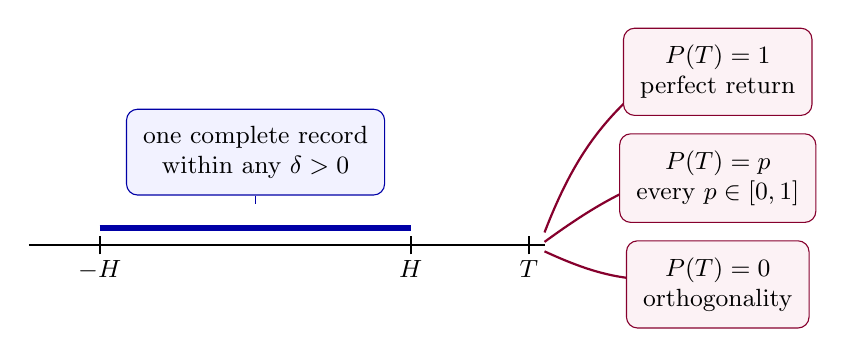
\begin{tikzpicture}[
  font=\small,
  arr/.style={-{Latex[length=2.2mm]},thick},
  box/.style={draw,rounded corners,align=center,inner sep=6pt},
  record/.style={draw=blue!65!black,fill=blue!5},
  outcome/.style={draw=purple!70!black,fill=purple!5}
]
\draw[thick] (-4.5,0)--(2.05,0);
\draw[thick] (-3.6,-0.12)--(-3.6,0.12);
\draw[thick] (0.35,-0.12)--(0.35,0.12);
\draw[thick] (1.85,-0.12)--(1.85,0.12);
\node[below=2pt] at (-3.6,0) {\(-H\)};
\node[below=2pt] at (0.35,0) {\(H\)};
\node[below=2pt] at (1.85,0) {\(T\)};
\draw[blue!65!black,line width=2.3pt] (-3.6,0.22)--(0.35,0.22);
\node[box,record] (record) at (-1.62,1.18)
  {one complete record\\within any \(\delta>0\)};
\draw[blue!65!black,dashed] (record.south)--(-1.62,0.48);
\draw[arr,purple!70!black] (2.05,0.16) to[bend left=14] (3.45,2.15);
\draw[arr,purple!70!black] (2.05,0.04) to[bend left=6] (3.45,0.85);
\draw[arr,purple!70!black] (2.05,-0.08) to[bend right=10] (3.45,-0.45);
\node[box,outcome] at (4.25,2.20) {\(P(T)=1\)\\perfect return};
\node[box,outcome] at (4.25,0.85) {\(P(T)=p\)\\every \(p\in[0,1]\)};
\node[box,outcome] at (4.25,-0.50) {\(P(T)=0\)\\orthogonality};
\end{tikzpicture}
\caption{\textbf{One observed return history permits every exact future
return probability.} Equivalently, one fixed state and return projector
evolve under isospectral nonnegative Hamiltonians. The record is one
survival probability, not full state tomography.}
\label{fig:law}
\end{figure}

Rescale time by \(t\mapsto t/T\), or equivalently replace
\(E_j\) by \(\pi j/T\). For any \(0\leq H<T\), set
\[
 s_H=\sin\left(\frac{\pi H}{2T}\right)<1 .
\]
Choosing \(n\) with \(2s_H^n<\delta\) proves uniform compatibility with the
single record \(P_0(t)\) throughout \([-H,H]\), simultaneously for every
\(p\in[0,1]\).

\section*{The universal law}

The construction also defeats any fixed finite list of local energy tests.
For \(k<n\), the finite-difference identity
\begin{equation}
 \sum_{j=0}^{n}(-1)^{n-j}{n\choose j}j^k=0
\label{eq:difference}
\end{equation}
implies
\begin{equation}
 \sum_{j=0}^{n}w_{p,j}E_j^k
 =\sum_{j=0}^{n}q_jE_j^k
 \quad\text{for every }p\in[0,1].
\label{eq:moments}
\end{equation}
Hence one may first prescribe any finite moment order \(m\), then choose
\(n>m\) large enough for the requested window precision.

\medskip
\noindent\textbf{Complete finite-horizon return ambiguity.}
\emph{For every \(m\in\mathbb N\), \(T>0\), \(0\leq H<T\), and
\(\delta>0\), there exist a finite-dimensional normalized state \(\phi\),
one record \(Q\) on \([-H,H]\), and a nonnegative self-adjoint Hamiltonian
\(\widetilde K_p\) for every \(p\in[0,1]\), such that all
\(\widetilde K_p\) are unitarily equivalent and:
\begin{enumerate}
\item \(\phi\) has the same energy moments through order \(m\) under every
      \(\widetilde K_p\);
\item with the fixed projector \(|\phi\rangle\langle\phi|\),
      \(\sup_{|t|\leq H}|P_p(t)-Q(t)|<\delta\) for every \(p\);
\item \(P_p(T)=p\) for every \(p\in[0,1]\).
\item for every \(p\in[0,1]\), \(\widetilde K_p\) may be chosen
      tridiagonal in the fixed basis; for \(p<1\) every adjacent path
      coupling of the Krylov representative is nonzero, whereas every
      tridiagonal fixed-protocol representative at \(p=1\) must have at
      least one zero path coupling.
\item for every fermion number \(k\), the canonical lifts
      \(\mathrm d\Gamma(\widetilde K_p)\) have a complete eigenbasis and
      one common subset-sum spectrum, including multiplicities.
\end{enumerate}}

The quantifiers matter. The horizon may approach \(T\) arbitrarily closely;
the error may be arbitrarily small but positive; the moment order may be
arbitrarily high but finite; and the target value is any and every allowed
probability. No infinite-dimensional limit, negative energy, random
Hamiltonian or computational assumption is used. In the dual representation
given above, all \(\widetilde K_p\) are replaced by the single uniform
qubit field \(H_{\rm u}\), and symmetric preparations vary instead.

\section*{Sharpness and forecasting consequence}

The moment ambiguity has a sharp support threshold. On \(r\) distinct
energy levels, the first \(r\) moments determine the \(r\) spectral weights:
their difference solves a square Vandermonde system. Therefore no two
different measures on at most \(n\) distinct levels can agree in all moments
of orders \(0,\ldots,n-1\). Equations~\eqref{eq:fullweight} and
\eqref{eq:parityweight} are different, agree in those \(n\) moment
constraints, and use \(n+1\) distinct levels. They attain the minimum
possible support.

Let \(F\) be any rule that maps the common record to a real forecast \(y\)
for \(P(T)\). The same input is compatible with \(p=0\) and \(p=1\), so
\begin{equation}
 \max\{|y|,|y-1|\}\geq\frac12.
\label{eq:minimax}
\end{equation}
This lower bound is independent of algorithm, training data architecture
and computational power. It does not shrink as \(\delta\downarrow0\) or
\(H\uparrow T\), provided the inequalities remain strict and dimension is
allowed to grow.

\section*{Meaning and experimental boundary}

The law is not indeterminism. If the exact Hamiltonian is known, unitary
dynamics fixes the future. Nor does the result concern full state or process
tomography. It isolates what one scalar but physically central
observable---return to one fixed initial state---can certify when the energy
levels are known but their eigenvectors are not.

The resource growth identifies how forecasting can recover. The construction
uses \(n+1\) levels and maximum angular energy \(\pi n/T\). A known
fixed resource bound independent of requested precision or a sufficiently
restricted Hamiltonian family can exclude the adversarial sequence.
Nearest-neighbour one-particle locality alone does not: every terminal
probability, including perfect return, has such a realization. The perfect
return construction uses a disconnected spectator block, and the rigidity
result proves that connected-path locality excludes this exact endpoint for
the fixed spectrum and preparation. It does not exclude any \(p<1\)
member, all of which have strictly positive spectral weights and an
irreducible Jacobi representative. Merely knowing the realized dimension,
bandwidth and complete spectrum does not distinguish members of each
constructed family. This explains why positive forecasting certificates
obtain their force from their model assumptions \cite{Valls2026,Manos2026}.

Spatial homogeneity alone is likewise insufficient in the dual protocol:
equations~\eqref{eq:uniformfield}--\eqref{eq:symmetricqubitstate} use one
fixed Hamiltonian invariant under every site permutation. There the
preparation carries the hidden spectral weights. This does not establish a
homogeneous fixed-preparation family; fixing both Hamiltonian and
preparation would of course fix the future.

Second quantization closes a different loophole: the candidates can be
placed inside full finite free-fermion Fock systems without changing any
particle-number-sector spectrum. It does not close the interaction or
thermodynamic-limit questions. The construction is inhomogeneous, its
couplings depend on \(p\), and no translationally invariant interacting
family is claimed.

The endpoint weights are binomial and parity-conditioned binomial
distributions, related to established binomial and even--odd binomial
states in quantum optics \cite{Stoler1985,Zhang2009}. Novelty claimed here
is therefore not a new state family. It is the universal forecasting law
and its fixed-protocol isospectral, nearest-neighbour and all-sector
free-fermion realization.
Platform-specific Hamiltonian synthesis, decoherence and measurement cost
are not part of the theorem and must be tested before an experimental claim.

The Loschmidt interpretation is equally precise. The \(p=0\) clock has a
real-time survival zero at \(T\); the \(p=1\) clock returns perfectly; all
intermediate probabilities occur under the same spectrum. A finite
Loschmidt zero is not automatically a thermodynamic-limit phase transition.
The conclusion is narrower and unconditional: a finite-window survival
record alone cannot certify whether such a zero, a perfect recurrence, or
any intermediate return will occur.

\section*{Methods}

\subsection*{Normalization and amplitude identities}

The binomial theorem normalizes \(q\). The alternating binomial sum at
degree zero normalizes \(r\) for \(n>0\), and convexity normalizes every
\(w_p\). Direct substitution gives
\[
\sum_j r_j z^j
=\left(\frac{1+z}{2}\right)^n+
\left(\frac{z-1}{2}\right)^n,
\]
which proves equations~\eqref{eq:A1} and \eqref{eq:Ap}. At
\(z=\ee^{\ii\pi}=-1\), the first term vanishes and the second is
\((-1)^n\), proving equation~\eqref{eq:allfutures}.

\subsection*{Uniform probability bound}

For real \(x\),
\[
\left|\frac{\ee^{\ii x}-1}{2}\right|=\left|\sin\frac{x}{2}\right|.
\]
This proves equation~\eqref{eq:exactdifference}. For complex \(a,b\) with
\(|a|,|b|\leq1\),
\[
\bigl||a|^2-|b|^2\bigr|
=\bigl||a|-|b|\bigr|(|a|+|b|)
\leq2|a-b|.
\]
All amplitudes are convex characteristic functions of probability
measures, hence have modulus at most one. Monotonicity of sine on
\([0,\pi/2]\) then proves equation~\eqref{eq:window}.

\subsection*{Moment identity and minimum support}

The \(n\)th forward difference annihilates every polynomial of degree below
\(n\), yielding equation~\eqref{eq:difference}. Multiplying by the common
energy scale and using equations~\eqref{eq:parityweight} and
\eqref{eq:interpolation} proves equation~\eqref{eq:moments}.

For the converse, let distinct energies \(x_0,\ldots,x_{r-1}\) support two
weight lists \(u,v\). Equality of moments of orders \(0,\ldots,r-1\) says
\[
\begin{pmatrix}
1&\cdots&1\\
x_0&\cdots&x_{r-1}\\
\vdots&&\vdots\\
x_0^{r-1}&\cdots&x_{r-1}^{r-1}
\end{pmatrix}(u-v)=0.
\]
The Vandermonde determinant is
\(\prod_{i<j}(x_j-x_i)\neq0\), so \(u=v\).

\subsection*{Statistics and reproducibility}

No statistical model, numerical fit or computed data enter the result. All
statements are exact identities or deterministic inequalities. The
Supplementary Information gives complete proofs and the scaled operational
form.

\subsection*{Data availability}

No datasets were generated or analysed.

\subsection*{Code availability}

No software is required to reproduce the analytic results.

\section*{End notes}

\textbf{Acknowledgements.} None.

\textbf{Funding.} No specific grant is associated with this work.

\textbf{Author contributions.} M.H. directed the study, developed the
mathematical argument and takes responsibility for all claims and text.

\textbf{Competing interests.} The author declares no competing interests.

\textbf{Additional information.} Supplementary Information is available for
this paper. Correspondence and requests for materials should be addressed to
M.H.

\begin{thebibliography}{99}

\bibitem{Rauer2018}
Rauer, B. \textit{et al.} Recurrences in an isolated quantum many-body
system. \textit{Science} \textbf{360}, 307--310 (2018).

\bibitem{KotowskiOszmaniec2026}
Kotowski, M. \& Oszmaniec, M. Tight bounds on recurrence time in closed
quantum systems. \textit{Phys. Rev. Lett.}, in press,
\url{https://doi.org/10.1103/crwj-qfw5} (2026).

\bibitem{GuptaShort2026}
Gupta, C. \& Short, A. J. Recurrence time for finite quantum systems.
Preprint at \url{https://arxiv.org/abs/2604.14995} (2026).

\bibitem{Karimi2026}
Karimi, B., Wu, X., Cleland, A. N. \& Pekola, J. P. Blueprint for
experiments exploring the quantum recurrence theorem on a coupled
multiqubit system. \textit{Phys. Rev. Res.} \textbf{8}, L012062 (2026).

\bibitem{Heyl2018}
Heyl, M. Dynamical quantum phase transitions: a review.
\textit{Rep. Prog. Phys.} \textbf{81}, 054001 (2018).

\bibitem{Zhou2021}
Zhou, B., Zeng, Y. \& Chen, S. Exact zeros of the Loschmidt echo and
quantum speed limit time for the dynamical quantum phase transition in
finite-size systems. \textit{Phys. Rev. B} \textbf{104}, 094311 (2021).

\bibitem{Novotny2026}
Novotn\'y, J., St\v{r}ele\v{c}ek, J., Str\'ansk\'y, P. \& Cejnar, P.
Tracing complex zeros of the quantum survival amplitude: how the energy
distribution controls dynamical phase transitions. Preprint at
\url{https://arxiv.org/abs/2605.06849} (2026).

\bibitem{Sornsaeng2024}
Sornsaeng, A., Dangniam, N. \& Chotibut, T. Quantum next generation
reservoir computing: an efficient quantum algorithm for forecasting quantum
dynamics. \textit{Quantum Mach. Intell.} \textbf{6}, 57 (2024).

\bibitem{Valls2026}
Valls, V. \textit{et al.} Forecasting quantum observables: a compressed
sensing approach with performance guarantees. \textit{Phys. Rev. Res.},
in press, \url{https://doi.org/10.1103/9qp3-33cs} (2026).

\bibitem{Manos2026}
Manos, K., Weilenmann, M. \& Navascu\'es, M. Timed demolition
measurements. Preprint at \url{https://arxiv.org/abs/2507.06912},
version 2 (2026).

\bibitem{ChenLi2026}
Chen, Z., Li, J. \& Slote, J. Lower bounds for learning Hamiltonians from
time evolution. Preprint at \url{https://arxiv.org/abs/2509.20665},
version 4 (2026).

\bibitem{Stoler1985}
Stoler, D., Saleh, B. E. A. \& Teich, M. C. Binomial states of the
quantized radiation field. \textit{Optica Acta} \textbf{32}, 345--355
(1985).

\bibitem{Zhang2009}
Zhang, X.-Y., Wang, J.-S., Meng, X.-G. \& Su, J. Wigner functions and
tomograms of the even and odd binomial states. \textit{Chin. Phys. B}
\textbf{18}, 604--610 (2009).

\bibitem{Chakrabarti2009}
Chakrabarti, R. \& Van der Jeugt, J. Quantum communication through a spin
chain with interaction determined by a Jacobi matrix.
\textit{J. Phys. A} \textbf{43}, 085302 (2010).

\bibitem{Bernard2025}
Bernard, P.-A., Cramp\'e, N., Labriet, Q., Morey, L. \& Vinet, L.
Exactly solvable inhomogeneous XY spin chain. Preprint at
\url{https://arxiv.org/abs/2507.06331} (2025).

\bibitem{Leite2005}
Leite, R. S., Saldanha, N. C. \& Tomei, C. Reconstruction of tridiagonal
matrices from spectral data. Preprint at
\url{https://arxiv.org/abs/math/0508099} (2005).

\end{thebibliography}

\end{document}
